
\documentclass[letterpaper, reqno,11pt]{article}
\usepackage[margin=1.0in]{geometry}
\usepackage{color,latexsym,amsmath,amssymb}
\usepackage{fancyhdr}
\usepackage{amsthm}
\usepackage{mathtools}
\usepackage{tikz}
\usepackage{float}
\usepackage{centernot}
\usepackage{subcaption}
\usepackage{extarrows}
\usetikzlibrary{hobby}
\usetikzlibrary{shapes.multipart}
\usepackage{pgfplots}
\pgfplotsset{compat=1.7}
\usetikzlibrary{arrows.meta}

\newcommand{\RR}{\mathbb{R}}
\newcommand{\CC}{\mathbb{C}}
\newcommand{\ZZ}{\mathbb{Z}}
\newcommand{\QQ}{\mathbb{Q}}
\newcommand{\NN}{\mathbb{N}}
\def\upint{\mathchoice%
  {\mkern13mu\overline{\vphantom{\intop}\mkern7mu}\mkern-20mu}%
  {\mkern7mu\overline{\vphantom{\intop}\mkern7mu}\mkern-14mu}%
  {\mkern7mu\overline{\vphantom{\intop}\mkern7mu}\mkern-14mu}%
  {\mkern7mu\overline{\vphantom{\intop}\mkern7mu}\mkern-14mu}%
  \int}
\def\lowint{\mkern3mu\underline{\vphantom{\intop}\mkern7mu}\mkern-10mu\int}
\DeclareMathOperator{\card}{card}
\DeclareMathOperator{\Binomial}{Binomial}
\pagestyle{fancy}
\lhead{Math 321 Lecture 17}
\rhead{Yuchong Pan}
\begin{document}
\pagenumbering{arabic}
\title{Math 321 Lecture 17}
\author{Yuchong Pan}
\date{February 11, 2019}
\newtheorem{thm}{Theorem}
\newtheorem{defn}{Definition}
\newtheorem*{remark}{Remark}
\newtheorem{claim}{Claim}
\newtheorem{cor}{Corollary}
\newtheorem{lemma}{Lemma}
\newtheorem{prop}{Proposition}
\maketitle
%

\section{Riemann-Stieltjes Integrals with General Integrators}

\begin{defn}
  \normalfont Suppose $f, \alpha : [a, b] \to \RR$, where $\alpha$ is not necessarily non-decreasing.

  \noindent {\bf Note:} Lower and upper Riemann sums need not obey the same inequalities as before.
  \begin{align*}
    L_\alpha (f, P) &= \sum_{i = 1}^n m_i \Delta \alpha_i, \\
    \centernot{\rotatebox[origin=c]{-90}{$\leq$}} \quad & \\
    U_\alpha (f, P) &= \sum_{i = 1}^n M_i \Delta \alpha_i.
  \end{align*}
  We have $m_i \leq M_i$, but $\Delta \alpha_i$ may not be $\geq 0$. Also note that $P \subseteq P'$ does not imply that $L_\alpha(f, P) \leq L_\alpha(f, P') \leq U_\alpha(f, P') \leq U_\alpha(f, P)$.

  Let $P = \{ a = x_0 < x_1 < \ldots < x_n = b \}$ be any partition of $[a, b]$. Choose a selection of points $T = \{ t_1 < t_2 < \ldots < t_n : t \in [x_{i - 1}, x_i] \}$.

  \begin{figure}[H]
    \centering
    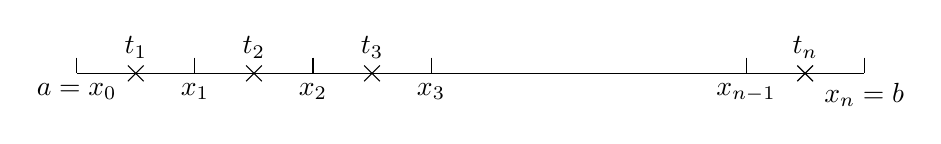
\begin{tikzpicture}
      \draw (0, 0) -- (10, 0);
      \draw (0, 0.2) -- (0, 0) node[below] {$a = x_0$};
      \draw (1.5, 0.2) -- (1.5, 0) node[below] {$x_1$};
      \draw (3, 0.2) -- (3, 0) node[below] {$x_2$};
      \draw (4.5, 0.2) -- (4.5, 0) node[below] {$x_3$};
      \draw (8.5, 0.2) -- (8.5, 0) node[below] {$x_{n - 1}$};
      \draw (10, 0.2) -- (10, 0) node[below] {$x_n = b$};
      \draw (0.65, -0.1) -- (0.85, 0.1);
      \draw (0.65, 0.1) -- (0.85, -0.1);
      \node[above, yshift=2pt] at (0.75, 0) {$t_1$};
      \draw (2.15, -0.1) -- (2.35, 0.1);
      \draw (2.15, 0.1) -- (2.35, -0.1);
      \node[above, yshift=2pt] at (2.25, 0) {$t_2$};
      \draw (3.65, -0.1) -- (3.85, 0.1);
      \draw (3.65, 0.1) -- (3.85, -0.1);
      \node[above, yshift=2pt] at (3.75, 0) {$t_3$};
      \draw (9.15, -0.1) -- (9.35, 0.1);
      \draw (9.15, 0.1) -- (9.35, -0.1);
      \node[above, yshift=2pt] at (9.25, 0) {$t_n$};
    \end{tikzpicture}
  \end{figure}

  Define
  $$ S_\alpha(f, P, T) = \sum_{i = 1}^n f(t_i) \Delta \alpha_i, \qquad \Delta \alpha_i = \alpha(x_i) - \alpha(x_{i - 1}). $$

  \begin{figure}[H]
    \centering
    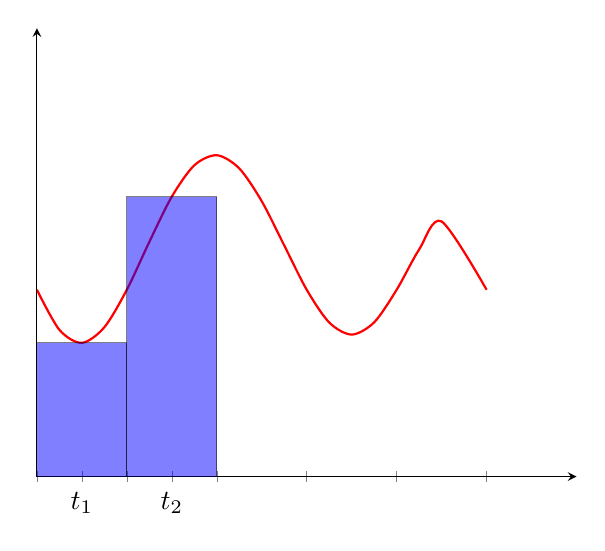
\begin{tikzpicture}[
        declare function={f(\x)=50000*(\x/2+0.3)*(\x/2+0.1)*(\x/2)*(\x/2-0.1)*(\x/2-0.3)*(\x/2-0.4)*(\x/2-0.5)*(\x/2-0.6)+0.5;},
      ]
      \begin{axis}[
          xmin=0,
          xmax=1.2,
          ymin=0,
          ymax=1.2,
          xtick={0, 0.1, 0.2, 0.3, 0.4, 0.6, 0.8, 1},
          xticklabels={, $t_1$, , $t_2$, , , , },
          ymajorticks=false,
          axis x line=bottom,
          axis y line=left,
        ]
        \addplot[thick, red, samples at={0, 0.05, ..., 0.95, 1}, smooth](x,{f(x)});
        \draw[fill=blue, opacity=0.5] (axis cs:0, 0) rectangle (axis cs:0.2, {f(0.1)});
        \draw[fill=blue, opacity=0.5] (axis cs:0.2, 0) rectangle (axis cs:0.4, {f(0.3)});
      \end{axis}
    \end{tikzpicture}
  \end{figure}

  We say that $f$ is {\bf RS-integrable} with respect to $\alpha$, written $f \in \mathcal R_\alpha[a, b]$, if there exists a real number $I$ such that for every $\epsilon > 0$, we can find a partition $P_0 = P_0(f, \alpha, \epsilon)$ such that $|S_\alpha(f, P, T) - I| < \epsilon$ for all partitions $P \supseteq P_0$ and any selection of points $T$. We write
  $$ I = \int_a^b fd\alpha. $$
\end{defn}

\noindent {\bf Exercise:} Check that for non-decreasing integrators $\alpha$, this definition is equivalent to our earlier one.

\section{Functions of Bounded Variation}

\subsection{Examples}

\noindent {\bf Recall:} A function $\alpha : [a, b] \to \RR$ is said to be of {\bf bounded variation}, written $\alpha \in BV[a, b]$, if
\begin{align*}
  & V_a^b \alpha = \text{{\bf total variation} of $\alpha$ on $[a, b]$} = \sup_P V_a^b (\alpha, P) < \infty, \\
  & \text{where } V_a^b(\alpha, P) = \sum_{i = 1}^n |\alpha(x_i) - \alpha(x_{i - 1})| = \sum_{i = 1}^n |\Delta \alpha_i|.
\end{align*}

\medskip

\noindent {\bf Examples:}
\begin{enumerate}
\item Constant functions are in $BV[a, b]$.
\item $BV[a, b] \subseteq \mathcal B[a, b] = \text{ space of bounded real-valued functions on $[a, b]$}$.

  Let $\alpha \in BV[a, b]$. Then,
  \begin{align*}
    |\alpha(x)| & \overset{\text{triangular inequality}}{\leq} \underbrace{|\alpha(x) - \alpha(a)|}_{|\Delta \alpha_1|} + |\alpha(a)| \\
    &\leq |\Delta \alpha_1| + |\Delta \alpha_2| + |\alpha(a)| \\
    &= V_a^b (\alpha, P) + |\alpha(a)| \\
    &\leq \underbrace{V_a^b \alpha + |\alpha(a)|}_\text{no dependence on $x$} \\
    &< \infty.
  \end{align*}

  \begin{figure}[H]
    \centering
    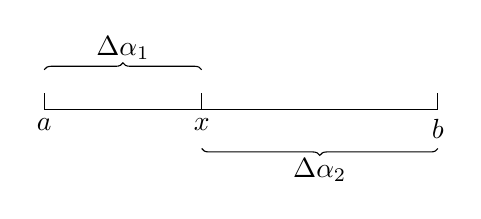
\begin{tikzpicture}
      \draw (0, 0) -- (5, 0);
      \draw (0, 0.2) -- (0, 0) node[below] {$a$};
      \draw (2, 0.2) -- (2, 0) node[below] {$x$};
      \draw (5, 0.2) -- (5, 0) node[below] {$b$};
      \draw[decoration={brace, raise=0.5cm}, decorate] (0, 0) -- (2, 0) node[midway, above, yshift=0.5cm] {$\Delta \alpha_1$};
      \draw[decoration={brace, mirror, raise=0.5cm}, decorate] (2, 0) -- (5, 0) node[midway, below, yshift=-0.5cm] {$\Delta \alpha_2$};
    \end{tikzpicture}
  \end{figure}
\item Not all bounded continuous functions in $[a, b]$ are in $BV[a, b]$.

  $$ \alpha(x) = \left\{
  \begin{array}{ll}
    x \sin\left(\frac{1}{x}\right), & \text{for $x \neq 0$}, \\
    0, & \text{at $x = 0$}.
  \end{array}
  \right. $$

  \begin{figure}[H]
    \centering
    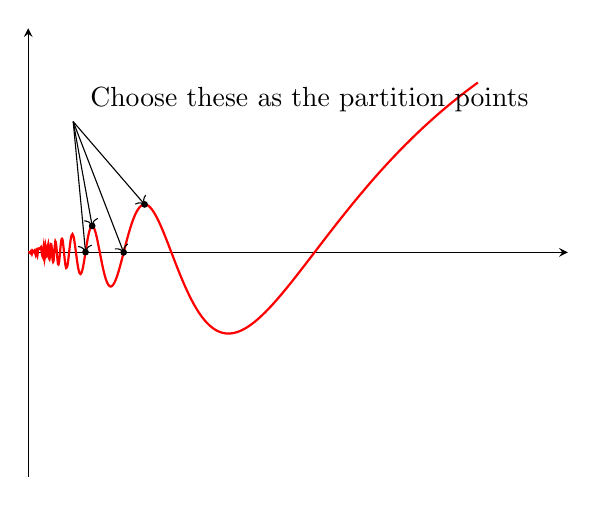
\begin{tikzpicture}[
        declare function={f(\x)=sin(deg(1/\x))*\x;},
      ]
      \begin{axis}[
          xmin=0,
          xmax=0.6,
          ymin=-0.6,
          ymax=0.6,
          xmajorticks=false,
          ymajorticks=false,
          axis x line=center,
          axis y line=left,
        ]
        \addplot[thick, red, domain=0.0001:0.5, samples=500, smooth](x,{f(x)});
        \draw[fill=black] (axis cs:0.1294, {f(0.1294)}) circle (1pt);
        \draw[fill=black] (axis cs:0.0711, {f(0.0711)}) circle (1pt);
        \draw[fill=black] (axis cs:0.1061, {f(0.1061)}) circle (1pt);
        \draw[fill=black] (axis cs:0.0637, {f(0.0637)}) circle (1pt);
        \draw[->] (axis cs:0.05, 0.35) -- (axis cs:0.1294, {f(0.1294)});
        \draw[->] (axis cs:0.05, 0.35) -- (axis cs:0.0711, {f(0.0711)});
        \draw[->] (axis cs:0.05, 0.35) -- (axis cs:0.1061, {f(0.1061)});
        \draw[->] (axis cs:0.05, 0.35) -- (axis cs:0.0637, {f(0.0637)});
        \node[above, xshift=3cm] at (axis cs:0.05, 0.35) {Choose these as the partition points};
      \end{axis}
    \end{tikzpicture}
  \end{figure}

  $\alpha \in C[a, b]$ for all $b > 0$, but $\alpha \not \in BV[a, b]$.
\item Any monotone function (increasing or decreasing, continuous or discontinuous) is in $BV[a, b]$.
\item Any step function with a finite number of jump discontinuities is in $BV[a, b]$.
\end{enumerate}

\subsection{Jordan's Theorem}

\begin{thm}[Jordan's theorem]
  \normalfont Any $\alpha \in BV[a, b]$ can be written as
  $$ \alpha = \beta - \gamma, $$
  where
  $\beta$ and $\gamma$ are both nondecreasing bounded functions on $[a, b]$.
\end{thm}

\begin{remark}
  \normalfont
  $$ \int_a^b fd\alpha \xlongequal{\text{Jordan's}} \int_a^b fd(\beta - \gamma) \xlongequal{\text{?}} \underbrace{\int_a^b fd\beta - \int_a^b fd\gamma}_\text{these are computable by our earlier discussion on non-decreasing integrators}. $$
\end{remark}

\end{document}
